\documentclass[11pt,a4paper,openany]{book}
\usepackage[margin=24mm]{geometry}
\usepackage{fontspec}
\IfFontExistsTF{Noto Serif}{\setmainfont{Noto Serif}}{\setmainfont{DejaVu Serif}}
\usepackage{amsmath,amssymb,tikz,enumitem,microtype}
\usepackage[hidelinks]{hyperref}
\setlength{\parindent}{0pt}
\setlength{\parskip}{6pt}
\setlist[enumerate]{leftmargin=*,itemsep=8pt}
\setlength{\emergencystretch}{2em}

\renewcommand{\contentsname}{Mục lục}
\begin{document}
\title{V-TALENT 2045\\ PHY101-A --- Đơn vị, tỉ lệ và đại số dành cho Vật lý\\\large Level 1 \textbar{} Mathematics for Physics}
\author{Dr. Dang Minh Tuan -- TS. Đặng Minh Tuấn}
\date{2026 \textbar{} Draft v1.0}
\maketitle
\tableofcontents
\chapter*{Hướng dẫn học}
Lớp 8–9. Học cách chuyển phép đo và phát biểu vật lý thành phương trình. Không yêu cầu giải tích. Tiên quyết: phân số, lũy thừa 10 và phương trình cơ bản.

Đọc mục tiêu và trả lời câu chẩn đoán trước lý thuyết. Tự tái lập lời giải ví dụ, giải độc lập bài luyện tập rồi dùng lời giải cuối sách để chẩn đoán lỗi. Dùng sổ riêng ghi dự đoán, sơ đồ và kiểm tra. Nội dung và bài tập tự biên soạn; nguồn ngoài là chỉ dẫn đọc, không sao chép. Bản thảo chờ thẩm định độc lập.
\chapter{Đo lường, hệ SI và suy luận thứ nguyên}
\section{Mục tiêu và chẩn đoán}
Đổi đơn vị hợp thành; suy ra đơn vị; phân biệt tính đúng thứ nguyên với tính đúng vật lý.

\textbf{Dự đoán:} Vì sao 1 cm\textsuperscript{2} bằng 0,0001 m\textsuperscript{2} chứ không phải 0,01 m\textsuperscript{2}? Công thức đúng thứ nguyên vẫn có thể sai không?
\section{Lý thuyết và suy dẫn}
Một phép đo biểu diễn giá trị số nhân với đơn vị. Đổi đơn vị làm đổi giá trị số, không đổi đại lượng vật lý. Các đơn vị cơ bản SI thường dùng ở đây là mét (m), kilôgam (kg), giây (s), ampe (A), kelvin (K), mol (mol); đơn vị thứ bảy là candela (cd). Một centimét bằng $10^{-2}$ m, milimét bằng $10^{-3}$ m, micromét bằng $10^{-6}$ m. Khi lũy thừa độ dài, phải lũy thừa cả hệ số đổi: $(1\,\mathrm{cm})^2=10^{-4}\,\mathrm{m^2}$ và $(1\,\mathrm{cm})^3=10^{-6}\,\mathrm{m^3}$.

Thứ nguyên mô tả loại đại lượng: độ dài $L$, khối lượng $M$, thời gian $T$. Tốc độ có thứ nguyên $LT^{-1}$, gia tốc $LT^{-2}$, lực $MLT^{-2}$, áp suất $ML^{-1}T^{-2}$ và năng lượng $ML^2T^{-2}$. Ví dụ $p=F/A$ dẫn tới $\mathrm{Pa=N/m^2}$; $W=Fs$ (lực không đổi cùng hướng) cho $\mathrm{J=N\,m}$. Lực và năng lượng không thể thay thế nhau dù giá trị số trùng nhau.

Hai vế của phương trình vật lý phải cùng thứ nguyên; các số hạng cộng hoặc trừ cũng phải cùng thứ nguyên. Vì vậy $s=vt+at^2$ vượt qua kiểm tra thứ nguyên, nhưng không đúng với độ dời khi gia tốc không đổi và $v$ là vận tốc đầu: số hạng thứ hai cần hệ số $1/2$. Phân tích thứ nguyên không xác định được hệ số không thứ nguyên hay chứng minh định luật vật lý. Nó giúp phát hiện lỗi, thu hẹp mô hình và định hướng phép đo.

Dùng phân số đổi đơn vị bằng một, như $1000\,\mathrm{m}/1\,\mathrm{km}$ và $1\,\mathrm{h}/3600\,\mathrm{s}$. Nhân cho đến khi đơn vị không mong muốn triệt tiêu. Với khối lượng riêng $\rho=m/V$, phải đổi cả khối lượng lẫn thể tích. Viết đơn vị ở từng bước. Giữ giá trị chưa làm tròn trong quá trình tính và làm tròn kết quả theo chất lượng dữ liệu.
\begin{center}
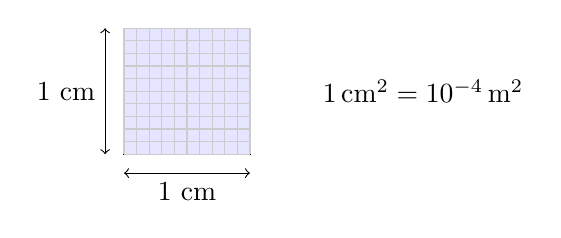
\begin{tikzpicture}[scale=.8]\draw[fill=blue!10] (0,0) rectangle (2,2);\draw[<->] (0,-.3)--node[below]{1 cm}(2,-.3);\draw[<->] (-.3,0)--node[left]{1 cm}(-.3,2);\draw[step=.2,gray!40] (0,0) grid (2,2);\node[right] at (3,1){$1\,\mathrm{cm^2}=10^{-4}\,\mathrm{m^2}$};\end{tikzpicture}
\end{center}
\section{Ví dụ có lời giải}
\subsection*{Ví dụ 1.1}
Đổi 54 km/h và 1,25 g/cm\textsuperscript{3} sang SI.

\textbf{Lời giải.} $54(1000/3600)=15$ m/s. Đồng thời $1{,}25(10^{-3})/(10^{-6})=1250$ kg/m$^3$. Hệ số đổi thể tích phải lấy lũy thừa ba.
\subsection*{Ví dụ 1.2}
Lực vuông góc 120 N tác dụng lên diện tích 30 cm\textsuperscript{2}. Tính áp suất theo Pa; giải thích vì sao chia cho 30 không cho giá trị SI.

\textbf{Lời giải.} $A=30\times10^{-4}=0{,}003$ m$^2$. Vậy $p=120/0{,}003=40000$ Pa. Thương chưa đổi bằng 4 có đơn vị N/cm$^2$, không phải Pa.
\subsection*{Ví dụ 1.3}
Biểu thức nào có thể biểu diễn thời gian: v/g, g/v hay v\textsuperscript{2}/g? v là tốc độ, g là gia tốc.

\textbf{Lời giải.} $[v/g]=(LT^{-1})/(LT^{-2})=T$. Biểu thức thứ hai là $T^{-1}$; thứ ba là $L$. Chỉ $v/g$ có thứ nguyên thời gian, nhưng hệ số và tính đúng vật lý vẫn cần mô hình.
\section{Nhiệm vụ thực nghiệm}
Đo các cạnh và khối lượng vật hộp ba lần. Tính thể tích và khối lượng riêng bằng SI và g/cm\textsuperscript{3}, rồi đổi đơn vị để đối chiếu. Báo độ chia thước và giải thích vì sao đo lặp không loại được lệch điểm 0.
\section{Ứng dụng hiện đại và chuyển giao}
Cảm biến áp suất MEMS chịu chênh lệch áp suất 2500 Pa trên màng có diện tích 4 mm$^2$. Với xấp xỉ áp suất đều, lực tổng hợp $F=pA=2500(4\times10^{-6})=0{,}010$ N. Vì vậy cảm biến vi chế tạo đòi hỏi đổi đơn vị và độ nhạy lực chính xác. Chuyển giao: nếu màng cùng hình dạng rộng gấp đôi, dự đoán lực; phân biệt lực với tín hiệu điện, vốn cần mô hình hiệu chuẩn riêng.
\section{Chỉ dẫn đọc nguồn}
SW-14: ch. 14, §§14.3–14.4, pp. 304–306; JP-1.1: p. 3; JP-1.2: p. 4 (check ratio direction); JP-1.5: p. 8 (extension).
\section{Luyện tập độc lập}
\begin{enumerate}
\item \textbf{PHY101-A-1.1}. Đổi 7,2 km/h sang m/s và 0,35 m\textsuperscript{2} sang cm\textsuperscript{2}.
\item \textbf{PHY101-A-1.2}. Khối lập phương cạnh 4 cm, khối lượng 172,8 g. Tính khối lượng riêng theo kg/m\textsuperscript{3}.
\item \textbf{PHY101-A-1.3}. Tải 48 N đặt trên bốn đệm bằng nhau, mỗi đệm 2 cm\textsuperscript{2}. Tính áp suất tiếp xúc trung bình.
\item \textbf{PHY101-A-1.4}. Cho F=ma và P=Fv, suy ra đơn vị cơ bản SI của công suất.
\item \textbf{PHY101-A-1.5}. Một biểu thức thế năng lò xo là kx, k có đơn vị N/m. Kiểm tra và đề xuất dạng đúng thứ nguyên chỉ dùng k và x.
\end{enumerate}
\chapter{Tỉ số, quan hệ tỉ lệ và quy luật đồng dạng}
\section{Mục tiêu và chẩn đoán}
Phân biệt tỉ lệ thuận, nghịch và luật lũy thừa; suy luận về diện tích, thể tích và đồng dạng.

\textbf{Dự đoán:} Nếu bán kính quả cầu tăng gấp đôi, khối lượng có tăng gấp đôi không? Điều gì phải giữ cố định?
\section{Lý thuyết và suy dẫn}
Với tỉ lệ thuận $y=kx$, thương $y/x$ không đổi; đồ thị là đường thẳng qua gốc. Đường thẳng $y=kx+b$ với $b\ne0$ không phải tỉ lệ thuận. Với tỉ lệ nghịch $y=k/x$, tích $xy$ không đổi. Mọi quan hệ tỉ lệ vật lý đều có điều kiện: $p\propto1/A$ chỉ khi giữ lực pháp tuyến; $I\propto V$ chỉ khi điện trở không đổi.

Luật lũy thừa $y=Cx^n$ cho $y_2/y_1=(x_2/x_1)^n$ khi $C$ không đổi. Các vật đồng dạng có hệ số độ dài $\lambda$, diện tích $\lambda^2$, thể tích $\lambda^3$. Nếu khối lượng riêng không đổi, khối lượng tỉ lệ thể tích. Vật chịu trọng lượng bản thân trên mặt tiếp xúc đồng dạng có áp suất tỉ lệ $\lambda^3/\lambda^2=\lambda$; vật lớn không đơn thuần là vật nhỏ phóng to mà ứng suất vẫn giữ nguyên.

Đại lượng hữu ích là tỉ số diện tích bề mặt trên thể tích. Với lập phương cạnh $l$, $A/V=6/l$. Với cầu bán kính $r$, $A/V=3/r$. Vật nhỏ có nhiều bề mặt hơn trên một đơn vị thể tích. Trong trao đổi nhiệt, phản ứng hóa học hay khuếch tán sinh học, tỉ số này quan trọng, nhưng tốc độ thực còn phụ thuộc vật liệu, chênh lệch nhiệt độ và điều kiện biên. Quy luật đồng dạng giải thích xu thế, không thay mô hình đầy đủ.
\begin{center}
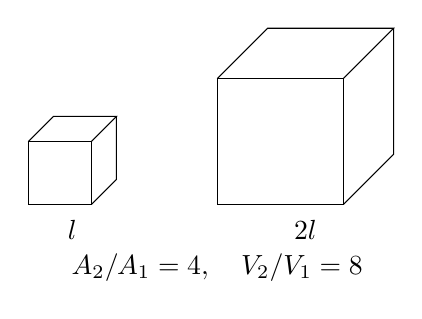
\begin{tikzpicture}[scale=.8]\draw (0,0) rectangle (1,1);\draw (0,1)--(.4,1.4)--(1.4,1.4)--(1,1);\draw (1,0)--(1.4,.4)--(1.4,1.4);\draw (3,0) rectangle (5,2);\draw (3,2)--(3.8,2.8)--(5.8,2.8)--(5,2);\draw (5,0)--(5.8,.8)--(5.8,2.8);\node at (.7,-.4){$l$};\node at (4.4,-.4){$2l$};\node at (3,-1){$A_2/A_1=4,\quad V_2/V_1=8$};\end{tikzpicture}
\end{center}
\section{Ví dụ có lời giải}
\subsection*{Ví dụ 2.1}
Điện trở có dòng 0,20 A khi điện áp 3 V. Dự đoán dòng ở 7,5 V nếu điện trở không đổi.

\textbf{Lời giải.} $I_2/I_1=7{,}5/3=2{,}5$; $I_2=0{,}50$ A. Tương đương $R=15\,\Omega$. Sự nóng lên có thể làm giả thiết mất hiệu lực.
\subsection*{Ví dụ 2.2}
Mô hình thuyền phóng to với hệ số độ dài 3, cùng khối lượng riêng. Khối lượng, diện tích boong tương ứng và trọng lượng trung bình trên diện tích boong thay đổi thế nào?

\textbf{Lời giải.} Khối lượng tăng $3^3=27$ lần; diện tích tăng $3^2=9$ lần; trọng lượng trên diện tích tăng $27/9=3$ lần. Đây là ước lượng đồng dạng, không phải phân bố ứng suất hoặc lực nổi cục bộ.
\subsection*{Ví dụ 2.3}
Đại lượng tuân theo y=Cx\textsuperscript{2}. Khi x từ 4 thành 10, y từ 12 thành bao nhiêu?

\textbf{Lời giải.} $y_2=12(10/4)^2=75$. Kiểm tra $C=12/16=0{,}75$ và $0{,}75(100)=75$.
\section{Nhiệm vụ thực nghiệm}
Lập bảng cạnh lập phương 1, 2, 4, 8 cm. Tính diện tích, thể tích và A/V. Vẽ A/V theo 1/l và giải thích độ dốc. Dùng SIM-M01 đối chiếu dự đoán.
\section{Ứng dụng hiện đại và chuyển giao}
Chia khối lập phương cạnh 12 mm thành $4^3=64$ khối cạnh 3 mm. Nếu mọi bề mặt đều lộ ra, tổng diện tích tăng từ $6(12)^2=864$ mm$^2$ lên $64(6)(3)^2=3456$ mm$^2$, gấp bốn; thể tích không đổi. Đây là một lý do kích thước hạt quan trọng trong xử lý vật liệu và xúc tác. Chuyển giao: dự đoán hệ số diện tích khi chia cạnh thành $n$ phần, giải thích vì sao hạt đóng chặt không lộ toàn bộ bề mặt.
\section{Chỉ dẫn đọc nguồn}
JP-1.5: dimensional scaling, p. 8; SW-14: dimensional analysis, p. 305.
\section{Luyện tập độc lập}
\begin{enumerate}
\item \textbf{PHY101-A-2.1}. Lò xo lý tưởng dãn 8 mm khi chịu 2 N. Dự đoán độ dãn ở 5 N trong miền tuyến tính.
\item \textbf{PHY101-A-2.2}. Lực 60 N tác dụng trên 0,020 m\textsuperscript{2}. Giảm diện tích một nửa, lực không đổi. Tìm hai áp suất.
\item \textbf{PHY101-A-2.3}. Hai cầu đặc đồng dạng bán kính 2 cm và 5 cm, cùng vật liệu. Tìm tỉ số khối lượng và diện tích (lớn/nhỏ).
\item \textbf{PHY101-A-2.4}. Ở tốc độ cố định, động năng tăng gấp đôi khi khối lượng gấp đôi. Giữ khối lượng, tốc độ tăng gấp ba thì sao?
\item \textbf{PHY101-A-2.5}. Hộp lập phương kín phóng to gấp 2. Nếu tốc độ tỏa nhiệt trên đơn vị diện tích như nhau và nhiệt dung tỉ lệ thể tích, so sánh tốc độ nguội ban đầu.
\end{enumerate}
\chapter{Đại số như công cụ mô hình hóa vật lý}
\section{Mục tiêu và chẩn đoán}
Biến đổi phương trình, giải hệ, chọn nghiệm có ý nghĩa vật lý và biểu diễn hiệu chuẩn tuyến tính.

\textbf{Dự đoán:} Một phương trình có hai nghiệm đại số. Cả hai có nhất thiết khả thi về vật lý không?
\section{Lý thuyết và suy dẫn}
Phương trình vật lý là ràng buộc giữa các đại lượng, không chỉ là công thức thế số. Biến đổi ký hiệu trước để thấy sự phụ thuộc. Từ $P=UI$ và $U=IR$ suy ra $P=I^2R=U^2/R$ đối với điện trở Ohm. Hai dạng cho xu thế khác nhau tùy giữ dòng hay điện áp. Trước khi chia một đại lượng phải kiểm tra nó khác 0.

Quan hệ tuyến tính có độ lệch dạng $y=ax+b$. Với hai đầu vào hiệu chuẩn khác nhau, $a=(y_2-y_1)/(x_2-x_1)$ và $b=y_1-ax_1$. Độ dốc có đơn vị đầu ra chia đầu vào, hệ số chặn có đơn vị đầu ra. Đảo quan hệ để hiệu chuẩn: $x=(y-b)/a$ nếu $a\ne0$. Nội suy trong miền đã đo thường đáng tin cậy hơn ngoại suy. Hai điểm luôn xác định một đường thẳng, nên cần dữ liệu bổ sung để kiểm tra tính tuyến tính.

Hệ phương trình xuất hiện khi nhiều điều kiện phải đồng thời thỏa. Trộn nhiệt lý tưởng với cùng nhiệt dung riêng, bỏ qua hao phí: $m_h(T_h-T)=m_c(T-T_c)$; suy ra $T=(m_hT_h+m_cT_c)/(m_h+m_c)$. Với khối lượng dương, nhiệt độ nằm giữa hai nhiệt độ đầu. Trong chuyển động, $s=ut+at^2/2$ có thể có hai nghiệm; dùng mốc thời gian, chiều, tiếp xúc và miền hiệu lực để chọn nghiệm đúng. Lời giải chỉ hoàn chỉnh khi thế kiểm tra và diễn giải vật lý.
\begin{center}
\begin{tikzpicture}[x=1.05cm,y=.7cm]\draw[->](0,0)--(5.3,0)node[right]{$x$};\draw[->](0,0)--(0,6)node[above]{$y$};\draw[thick,blue](0,1)--(4.5,5.5);\fill (1,2)circle(2pt) (4,5)circle(2pt);\draw[dashed](1,2)--(4,2)--(4,5);\node at (2.5,1.7){$\Delta x$};\node[right]at(4,3.5){$\Delta y$};\node[left]at(0,1){$b$};\end{tikzpicture}
\end{center}
\section{Ví dụ có lời giải}
\subsection*{Ví dụ 3.1}
Cảm biến đọc 0,40 V tại 0 N và 2,40 V tại 10 N. Giả sử đáp ứng tuyến tính, ước lượng lực tại 1,60 V.

\textbf{Lời giải.} $a=(2{,}40-0{,}40)/10=0{,}20$ V/N; $U=0{,}40+0{,}20F$. Vậy $F=(1{,}60-0{,}40)/0{,}20=6$ N, nằm trong miền hiệu chuẩn.
\subsection*{Ví dụ 3.2}
Trộn 200 g nước 65\textdegree{}C với 300 g nước 15\textdegree{}C trong bình cách nhiệt lý tưởng. Tìm nhiệt độ cân bằng.

\textbf{Lời giải.} Nhiệt dung riêng bằng nhau nên triệt tiêu: $200(65-T)=300(T-15)$. Suy ra $500T=17500$, $T=35^\circ$C. Kết quả gần nhiệt độ của khối lượng lớn hơn.
\subsection*{Ví dụ 3.3}
Vật có x=3t\textsuperscript{2}-6t (m), t\ensuremath{\ge}0. Khi nào vật ở x=9 m?

\textbf{Lời giải.} $3t^2-6t-9=0$ cho $(t-3)(t+1)=0$. Hai nghiệm 3 s và -1 s; loại -1 do miền $t\ge0$. Kiểm tra $x(3)=9$ m.
\section{Nhiệm vụ thực nghiệm}
Dùng lò xo và quả cân nhỏ đã biết một cách an toàn. Vẽ độ dãn theo tải; ước lượng độ dốc từ các điểm cách xa rồi kiểm tra điểm giữa. Nếu lò xo không trở về chiều dài ban đầu, dừng: mô hình đàn hồi không còn đáng tin.
\section{Ứng dụng hiện đại và chuyển giao}
Với thiết bị ghi nhiệt độ dùng pin, cảm biến tuyến tính có thể cho 0,50 V tại 0\textdegree{}C và 0,90 V tại 40\textdegree{}C. Độ dốc hiệu chuẩn 0,010 V/\textdegree{}C; đầu ra 0,73 V ứng với 23\textdegree{}C. Chuyển giao: độ lệch điểm 0 tăng 0,020 V làm kết quả cao hơn 2\textdegree{}C nếu bỏ qua. Giải thích cách phát hiện bằng nhiệt kế chuẩn và vì sao cảm biến thực cần kiểm tra ở hơn hai mức nhiệt.
\section{Chỉ dẫn đọc nguồn}
SJ-01: Functions, p. 9 (selected reading; calculus deferred); SW-14: graphs, pp. 305–306; JP-C7: linear fit, pp. 288–292 (teacher extension).
\section{Luyện tập độc lập}
\begin{enumerate}
\item \textbf{PHY101-A-3.1}. Nguồn 12 V cấp điện trở lý tưởng 6 \ensuremath{\Omega}. Tìm dòng, công suất; sau đó tăng điện trở gấp đôi với điện áp cố định.
\item \textbf{PHY101-A-3.2}. Cảm biến lực đọc 0,6 V tại 2 N và 1,8 V tại 8 N. Tìm phương trình tuyến tính và lực tại 1,2 V.
\item \textbf{PHY101-A-3.3}. Cần bao nhiêu nước 80\textdegree{}C trộn với 150 g nước 20\textdegree{}C để đạt 40\textdegree{}C, bỏ qua hao phí?
\item \textbf{PHY101-A-3.4}. Hai vật có tổng khối lượng 500 g và chênh lệch 80 g. Tìm khối lượng từng vật.
\item \textbf{PHY101-A-3.5}. Vật chuyển động theo x=2t\textsuperscript{2}+2t với t\ensuremath{\ge}0. Tìm thời điểm x=12 m.
\end{enumerate}
\chapter{Ước lượng, bất định và kiểm tra mô hình}
\section{Mục tiêu và chẩn đoán}
Ước lượng bậc độ lớn, phân biệt độ phân giải với độ đúng và so sánh dự đoán với quan sát.

\textbf{Dự đoán:} Máy tính cho 3,14159265 thì thí nghiệm có bảo đảm được tất cả chữ số đó không?
\section{Lý thuyết và suy dẫn}
Ước lượng bậc độ lớn xác định quy mô hợp lý trước khi tính chi tiết. Chia đại lượng chưa biết thành các yếu tố có thể đo hoặc ước lượng có căn cứ. Ví dụ thể tích phòng từ dài, rộng, cao; nhân với khối lượng riêng không khí giả định để ước lượng khối lượng. Ghi giả thiết và phân biệt đại lượng đo với ước lượng. Nếu kết quả thay đổi mạnh khi giả thiết bất định thay đổi nhẹ, cần bằng chứng tốt hơn cho giả thiết đó.

Độ phân giải là bước hiển thị nhỏ nhất của dụng cụ. Độ đúng liên quan mức gần giá trị chuẩn hoặc giá trị thực; độ chụm liên quan sự phù hợp giữa các lần đo. Phép đo lặp có thể chụm nhưng không đúng do sai lệch hệ thống. Với cận đơn giản trong lớp, biểu diễn phép đo dương $x\pm\delta x$ và dùng giá trị nhỏ nhất/lớn nhất có thể. Cận này không mặc nhiên là độ lệch chuẩn hay khoảng tin cậy.

Nếu $z=xy$ và hai biến dương, cận là $(x-\delta x)(y-\delta y)$ và $(x+\delta x)(y+\delta y)$. Với $z=x/y$ và $y-\delta y>0$, cận dưới dùng tử nhỏ nhất, mẫu lớn nhất; cận trên làm ngược lại. So sánh dự đoán mô hình với cận đo; chênh lệch có thể do mô hình sai, bất định chưa tính hoặc lỗi phép đo. Phù hợp không chứng minh mô hình là lời giải thích duy nhất.
\begin{center}
\begin{tikzpicture}[x=.8cm]\draw[->](0,0)--(8,0)node[right]{$x$};\draw[thick,blue](1,1)--(5,1);\draw(1,.8)--(1,1.2)(5,.8)--(5,1.2);\fill(3,1)circle(2pt);\node[above]at(3,1.3){$x\pm\delta x$};\draw[thick,dashed](4,0)--(4,2);\node[above]at(4,2){$x_{\rm model}$};\end{tikzpicture}
\end{center}
\section{Ví dụ có lời giải}
\subsection*{Ví dụ 4.1}
Ước lượng khối lượng không khí trong phòng 5 m \ensuremath{\times} 4 m \ensuremath{\times} 3 m, dùng khối lượng riêng 1,2 kg/m\textsuperscript{3}.

\textbf{Lời giải.} $V=60$ m$^3$, $m=1{,}2(60)=72$ kg. Giả sử khối lượng riêng đều và bỏ qua thể tích đồ đạc; bậc độ lớn khoảng $10^2$ kg.
\subsection*{Ví dụ 4.2}
Hình chữ nhật đo được hai cạnh 10,0\ensuremath{\pm}0,1 cm và 5,0\ensuremath{\pm}0,1 cm. Tìm diện tích và cận cực trị.

\textbf{Lời giải.} Giá trị trung tâm $A=50{,}0$ cm$^2$. Cận dưới $9{,}9(4{,}9)=48{,}51$; trên $10{,}1(5{,}1)=51{,}51$ cm$^2$. Khoảng hơi bất đối xứng; cận làm tròn bảo thủ khoảng $50{,}0\pm1{,}6$ cm$^2$.
\subsection*{Ví dụ 4.3}
Nhiệt kế liên tục đọc 24,8\textdegree{}C trong bể chuẩn 25,0\textdegree{}C. Giải thích đo lặp nhất quán chứng tỏ điều gì và không chứng tỏ điều gì.

\textbf{Lời giải.} Các số đọc cho thấy độ lặp tốt ở độ phân giải hiển thị. Chúng lệch chuẩn -0,2\textdegree{}C. Có thể có lệch hệ thống, nhưng phải kiểm tra bất định chuẩn và điều kiện khác; độ lặp không đủ chứng minh độ đúng.
\section{Nhiệm vụ thực nghiệm}
Ước lượng thể tích lớp học bằng bước chân rồi đo bằng thước dây. So sánh hai ước lượng, liệt kê ít nhất ba nguồn bất định. Không coi kết quả thước dây là tuyệt đối chính xác.
\section{Ứng dụng hiện đại và chuyển giao}
Thiết bị ghi dữ liệu dùng năng lượng mặt trời tiêu thụ 0,30 W trong 24 giờ, tức 7,2 Wh/ngày. Tấm pin nhỏ cấp trung bình 2 W trong 4 giờ nắng hiệu dụng cho 8 Wh. Với hiệu suất lưu trữ/chuyển đổi 75 phần trăm, năng lượng dùng được 6 Wh, thiếu 1,2 Wh. Chuyển giao: tìm công suất trung bình tối thiểu theo giả thiết; giải thích vì sao thời tiết biến đổi và lão hóa pin cần dung lượng dự phòng.
\section{Chỉ dẫn đọc nguồn}
SW-14: §§14.1–14.4, pp. 301–306; JP-C7: §§7.1–7.5, pp. 273–292.
\section{Luyện tập độc lập}
\begin{enumerate}
\item \textbf{PHY101-A-4.1}. Ước lượng khối lượng tấm nhôm 2 m \ensuremath{\times} 1 m \ensuremath{\times} 1 mm, khối lượng riêng 2700 kg/m\textsuperscript{3}.
\item \textbf{PHY101-A-4.2}. Quãng đường 20,0\ensuremath{\pm}0,2 m và thời gian 4,0\ensuremath{\pm}0,1 s. Tìm tốc độ và cận cực trị.
\item \textbf{PHY101-A-4.3}. Thước luôn cộng 0,3 cm vào số đo trực tiếp. Mười lần đo trung bình 12,4 cm. Nếu biết chính xác độ lệch, hiệu chỉnh trung bình.
\item \textbf{PHY101-A-4.4}. Mô hình dự đoán 8,0 N; lực đo 7,4\ensuremath{\pm}0,2 N. Dự đoán có nằm trong cận không? Cần kiểm tra gì?
\item \textbf{PHY101-A-4.5}. Với thiết bị ghi dữ liệu mặt trời ở trên, tìm công suất pin trung bình tối thiểu trong bốn giờ nắng hiệu dụng, hiệu suất 75 phần trăm.
\end{enumerate}
\chapter*{Tài liệu tham khảo và mô phỏng}
Swiss Physics Olympiad Script, 3rd ed. (2019).\par
The Committee of Japan Physics Olympiad (2014). \textit{Physics Olympiad: Basic to Advanced Exercises}. World Scientific.\par
Tan Chien Hao (2024). \textit{Freshman Physics}.\par
\url{https://diavn.github.io/truongchuyen/physics-curriculum.html}\par
\url{https://diavn.github.io/truongchuyen/physics-math-lab.html}
\appendix
\chapter{Lời giải đầy đủ phần luyện tập}
\section{Đo lường, hệ SI và suy luận thứ nguyên}
\begin{enumerate}
\item \textbf{PHY101-A-1.1}. $7{,}2/3{,}6=2$ m/s; $0{,}35\times10^4=3500$ cm$^2$.
\item \textbf{PHY101-A-1.2}. $V=64$ cm$^3$; $\rho=172{,}8/64=2{,}7$ g/cm$^3=2700$ kg/m$^3$.
\item \textbf{PHY101-A-1.3}. Tổng diện tích $8\times10^{-4}$ m$^2$; $p=48/(8\times10^{-4})=60000$ Pa. Nếu tải phân bố đều, mỗi đệm chịu cùng áp suất.
\item \textbf{PHY101-A-1.4}. $[F]=MLT^{-2}$; nhân $LT^{-1}$ được $ML^2T^{-3}$, nên W = kg m$^2$ s$^{-3}$.
\item \textbf{PHY101-A-1.5}. $kx$ có đơn vị lực. $kx^2$ có đơn vị năng lượng; định luật lò xo lý tưởng là $U=kx^2/2$ tính từ trạng thái không biến dạng, suy từ công chứ không chỉ đơn vị.
\end{enumerate}
\section{Tỉ số, quan hệ tỉ lệ và quy luật đồng dạng}
\begin{enumerate}
\item \textbf{PHY101-A-2.1}. $x_2=8(5/2)=20$ mm.
\item \textbf{PHY101-A-2.2}. $p_1=60/0{,}020=3000$ Pa; $p_2=60/0{,}010=6000$ Pa.
\item \textbf{PHY101-A-2.3}. $\lambda=5/2$; tỉ số khối lượng $(5/2)^3=125/8$; diện tích $(5/2)^2=25/4$.
\item \textbf{PHY101-A-2.4}. $K=mv^2/2$, nên $K_2/K_1=3^2=9$.
\item \textbf{PHY101-A-2.5}. Công suất mất nhiệt tăng 4 lần; nhiệt dung tăng 8 lần. Tốc độ nguội ban đầu bằng công suất chia nhiệt dung nên giảm còn một nửa. Ở Level 1 hiểu là độ giảm nhiệt độ trong khoảng thời gian ngắn.
\end{enumerate}
\section{Đại số như công cụ mô hình hóa vật lý}
\begin{enumerate}
\item \textbf{PHY101-A-3.1}. $I=12/6=2$ A, $P=24$ W. Khi $R=12\,\Omega$, $I=1$ A, $P=12$ W.
\item \textbf{PHY101-A-3.2}. $a=(1{,}8-0{,}6)/6=0{,}2$ V/N; $b=0{,}6-0{,}2(2)=0{,}2$ V. $F=(1{,}2-0{,}2)/0{,}2=5$ N.
\item \textbf{PHY101-A-3.3}. $m(80-40)=150(40-20)$, nên $40m=3000$, $m=75$ g.
\item \textbf{PHY101-A-3.4}. $m_1+m_2=500$, $m_1-m_2=80$. Cộng: $2m_1=580$; $m_1=290$ g, $m_2=210$ g.
\item \textbf{PHY101-A-3.5}. $t^2+t-6=(t+3)(t-2)=0$. Nhận 2 s, loại -3 s.
\end{enumerate}
\section{Ước lượng, bất định và kiểm tra mô hình}
\begin{enumerate}
\item \textbf{PHY101-A-4.1}. $V=2(1)(0{,}001)=0{,}002$ m$^3$; $m=5{,}4$ kg.
\item \textbf{PHY101-A-4.2}. Trung tâm 5,0 m/s; dưới $19{,}8/4{,}1\approx4{,}83$; trên $20{,}2/3{,}9\approx5{,}18$ m/s.
\item \textbf{PHY101-A-4.3}. $12{,}4-0{,}3=12{,}1$ cm. Lấy trung bình không loại lệch; vẫn còn các bất định khác.
\item \textbf{PHY101-A-4.4}. Cận 7,2–7,6 N không chứa 8,0 N. Kiểm tra hiệu chuẩn, lực bỏ qua và bất định của dự đoán; không vội kết luận định luật sai.
\item \textbf{PHY101-A-4.5}. $0{,}75P(4)=7{,}2$ Wh, nên $P=2{,}4$ W. Chỉ vừa cân bằng năng lượng ngày theo mô hình, không có dự phòng.
\end{enumerate}
\end{document}
